\documentclass[12pt,a4paper]{scrartcl}
\usepackage[utf8]{inputenc}
\usepackage[english,russian]{babel}
\usepackage{indentfirst}
\usepackage{misccorr}
\usepackage{graphicx}
\usepackage{amsmath}
\usepackage{multirow}
\usepackage{pgfplots}
\usepackage{parskip}
\usepackage[top=1cm, bottom=1cm, left=1cm, right=1cm]{geometry}
\pgfplotsset{compat=1.9}

\begin{document}
	\graphicspath{{pic/}, {~/Pictures/TeXImgs/}}
	
	\newcommand{\ms}{\mathstrut}
	\newcommand{\msp}{\hspace{0.5cm}}
	\newcommand{\al}{\alpha}
	\newcommand{\dg}{^\circ}
	\newcommand{\dif}{\mathrm{d}}
	\newcommand{\qd}[2]{^{\frac{#1}{#2}}}
	\newcommand{\qdm}[2]{^{-\frac{#1}{#2}}}
	\newcommand{\lm}[2]{\underset{#1 \rightarrow #2}{\lim}}
	\newcommand{\sfrac}[2]{\dfrac{\strut #1}{\strut #2}}
	\newcommand{\equal}[1]{\overset{(#1)}{=}}
	\newcommand{\linevdots}{\ \raisebox{-.08\height}{\vdots}\ }
	\newcommand{\linecvdots}{\ \raisebox{-.08\height}{\vdots}\hspace{-0.13cm}\raisebox{.15\height}{\cancel{\phantom{a}}\hspace{0.06cm}}}
	\newcommand{\combox}[1]{\ms \msp \msp \begin{minipage}{0.95\linewidth}
			#1
	\end{minipage}}
	
	\newtheorem{pr}{Задача}
	\newtheorem{ex}{Пример}
	\newtheorem{dfn}{Def}
	\newtheorem{theorem}{Th}
	
	\newenvironment{slv}{\ms \msp \textit{Решение:}}{}
	\newenvironment{proof}{\ms \msp \textit{Доказательство: }}{\hfill $\square$}
	
	\begin{titlepage}
		
		\vspace*{\fill}
		
		\begin{center}
			
\includegraphics[scale=0.8]{MIPT.png}
			\\[0.7cm]\Huge Московский Физико-Технический Институт\\(национальный исследовательский университет)
			\\[2cm]\LARGE Отчет по эксперименту
			\\[0.5cm]\noindent\rule{\textwidth}{1pt}
			\\\Huge\textbf{Поляризация}
			\\[-0.5cm]\noindent\rule{\textwidth}{1pt}
		\end{center}
		
		\begin{flushleft}
			\textit{Работа №4.7.3; дата: 18.02.23}\hfill\textit{Семестр: 4}
		\end{flushleft}
		
		\vspace*{\fill}
		
		\begin{flushleft}
			Выполнил: \hspace{\fill} Группа:
			\\Кошелев Александр \hspace{\fill} Б05-105
		\end{flushleft}
	\end{titlepage}
	
	%Страница 2
	
	\begin{flushleft}
		\footnotesize{Поляризация} \hspace{\fill} \footnotesize{2}
		\\[-0.3cm]\noindent\rule{\textwidth}{0.3pt}
	\end{flushleft}
	
	\section{Аннотация}
	
	\textbf{Цель работы: }
	
	Ознакомление с методами получения и анализа поляризованного света.
		
	\textbf{В работе используются:}
	
	Оптическая скамья с осветителем; зелёный светофильтр; два поляроида; чёрное зеркало; полированная эбонитовая пластинка; стопа стеклянных пластинок; слюдяные пластинки разной толщины; пластинки в 1/4 и 1/2 длины волны; пластинка в одну длину волны для зелёного света (пластинка чувствительного оттенка).
	
	\section{Теоретические сведения}
	
	\subsection{Определение направления разрешённой плоскости колебаний поляроида}
	
	Определить направление разрешённых колебаний поляроида проще всего с помощью чёрного зеркала.
	
	При падении света на отражающую поверхность под углом Брюстера, свет в отражённом луче почти полностью поляризован, а вектор $\vec{E}$ параллелен отражающей поверхности ("<правило иголки">). Луч света,
	прошедший поляроид и отразившийся от чёрного зеркала, имеет минимальную интенсивность при выполнении двух условий: во-первых, свет падает на отражающую поверхность под углом Брюстера и, во-вторых,
	в падающем пучке вектор $\vec{E}$ лежит в плоскости падения.
	
	Вращая поляроид вокруг направления луча и чёрное зеркало вокруг
	оси, перпендикулярной лучу, методом последовательных приближений
	можно добиться минимальной яркости луча, отражённого от зеркала,
	и таким образом определить разрешённое направление поляроида.
	
	Измеряя угол поворота зеркала (угол Брюстера), нетрудно определить коэффициент преломления материала, из которого изготовлено
	зеркало. Описанный метод часто используется для измерения коэффициента преломления непрозрачных диэлектриков.
	
	\subsection{Получение эллиптически поляризованного света}
	
	\begin{center}
		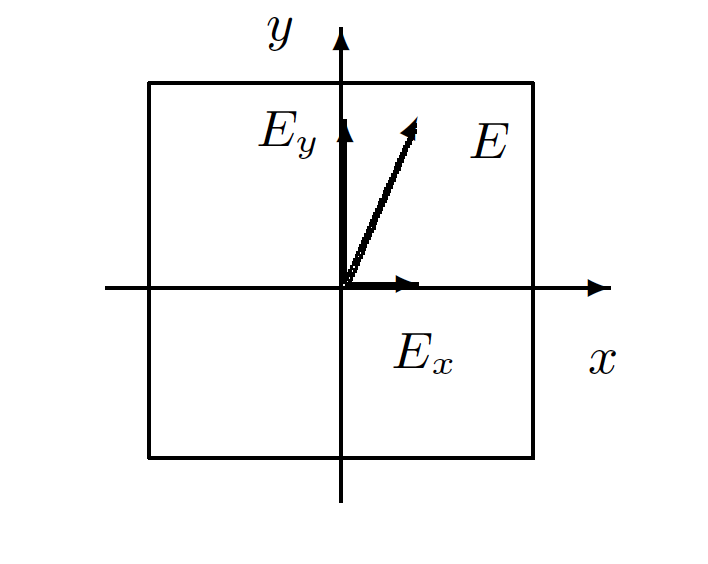
\includegraphics[scale=0.5]{PIC_1.png}
		\\\textbf{Рис. 1:} Разложение линейно поляризованного света по главным направлениям двоякопреломляющей пластинки
	\end{center}
	
	Эллиптически поляризованный свет можно получить из линейно поляризованного с
	помощью двоякопреломляющих кристаллических пластинок.
	
	\newpage
	
	%Страница 3
	
	\begin{flushleft}
		\footnotesize{Поляризация} \hspace{\fill} \footnotesize{3}
		\\[-0.3cm]\noindent\rule{\textwidth}{0.3pt}
	\end{flushleft}
	
	Двоякопреломляющая пластинка имеет два взаимно перпендикулярных главных направления, совпадающих с осями эллипсоида диэлектрической проницаемости. Волны, поляризованные вдоль главных направлений, распространяются в пластинке с разными скоростями, не изменяя характера своей поляризации. Эти волны называются главными. Мы будем обозначать показатели преломления для главных волн через $ n_x $ и $ n_y $, где $ x $ и $ y $ -- главные направления кристаллической пластинки (рис. 1).
	
	Пусть на пластинку падает линейно поляризованная волна, электрический вектор которой ориентирован под некоторым углом $\alpha$ к оси $x$. Разложим вектор $\vec{E}$ на составляющие $\vec{E_x}$ и $\vec{E_y}$. На входе пластинки $\vec{E_x}$ и $\vec{E_y}$ находятся в фазе. На выходе из-за разности скоростей между ними появляется разность хода $ d(n_x - n_y) $, при этом сдвиг фаз определяется соотношением
	
	$$\Delta \varphi = k d(n_x - n_y)$$	
	
	Как уже отмечалось, при сложении двух взаимно перпендикулярных колебаний, обладающих некоторым сдвигом фаз, образуется колебание, поляризованное по эллипсу.
	
	Рассмотрим практически важные частные случаи.
	
	\begin{enumerate}
		
		\item Пластинка даёт сдвиг фаз $ 2\pi $ (пластинка в длину волны $ \lambda $). В результате сложения волн на выходе пластинки образуется линейно поляризованная волна с тем же направлением колебаний, что и в падающей волне.
		
		\item Пластинка даёт сдвиг фаз $ \pi $ (пластинка в полдлины волны $ \lambda / 2 $). На выходе пластинки снова образуется линейно поляризованная волна. Направление $ bb' $ колебаний этой волны повёрнуто относительно направления $ aa' $ колебаний падающей волны (рис. 2). Как нетрудно сообразить, направление $ bb' $ является зеркальным отображением направления $ aa' $ относительно одного из главных направлений пластинки. Такую пластинку используют для поворота направления колебаний линейно поляризованного света.
		
		\item Пластинка создаёт между колебаниями сдвиг фаз $ \pi/2 $ (пластинка
		в четверть длины волны). При сложении двух взаимно перпендикулярных колебаний, имеющих разность фаз $ \pi/2 $, образуется эллипс, главные оси которого совпадают с координатными осями $ x $ и $ y $. При равенстве амплитуд возникает круговая поляризация.
		
	\end{enumerate}
	
	\begin{center}
		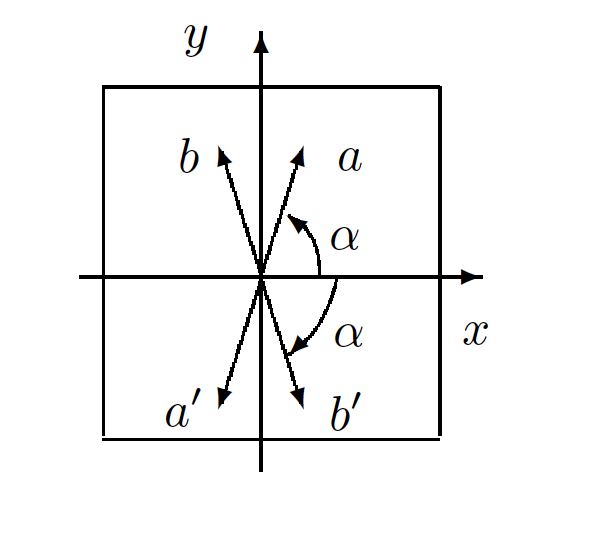
\includegraphics[scale=0.5]{PIC_2.png}
		\\\textbf{Рис. 2:} Поворот направления колебаний с помощью пластинки в $ \lambda / 2 $
	\end{center}
	
	Следует отметить, что, говоря о пластинках $ \lambda , \lambda/2, \lambda/4  $ и т. д., всегда подразумевают какую-либо вполне определённую монохроматическую
	компоненту (например, пластинка $ \lambda/2 $ для зелёного света). Если на двоякопреломляющую пластинку падает не монохроматический свет, то на
	выходе из неё для разных спектральных компонент эллипсы поляризации будут различными.
	
	\newpage
	
	%Страница 4
	
	\begin{flushleft}
		\footnotesize{Поляризация} \hspace{\fill} \footnotesize{4}
		\\[-0.3cm]\noindent\rule{\textwidth}{0.3pt}
	\end{flushleft}
	
	\subsection{Анализ эллиптически поляризованного света}
	
	Анализ эллиптически поляризованного света сводится к нахождению главных осей эллипса поляризации и к определению направления вращения электрического вектора.
	
	Главные оси эллипса поляризации определяются с помощью анализатора по максимуму и минимуму интенсивности проходящего света.
	Направление вращения электрического вектора может быть найдено
	с помощью пластинки в четверть длины волны, для которой известно,
	какая из главных волн, $ E_x $ или $ E_y $, имеет б\'{o}льшую скорость распространения (и соответственно меньшее значение показателя преломления).
	
	Выберем для определённости координатные оси x и y на пластинке
	так, чтобы $ n_x < n_y $. В этом случае главная волна $ E_x $ имеет большую
	скорость распространения. Поместим такую пластинку на пути эллиптически поляризованного света и совместим главные направления пластинки $ \lambda/4 $ с главными осями эллипса поляризации. На выходе из этой пластинки сдвиг фаз между $ E_x $ и $ E_y $ вместо $ \pi/2 $ станет равным нулю или $ \pi $. Свет окажется линейно поляризованным. Из двух возможных значений сдвига фаз, 0 или $ \pi $, реализуется одно: то, которое соответствует имеющемуся в волне направлению вращения электрического вектора.
	
	Рассмотрим, например, случай, когда электрический вектор в эллиптически поляризованной волне вращается против часовой стрелки,
	если смотреть навстречу лучу. В этом случае, очевидно, в волне, падающей на пластинку в $ \lambda/4 $, колебание $ E_y $ отстаёт по фазе на $ \pi/2 $ от
	колебания $ E_x $. При прохождении через пластинку разность фаз увеличивается до $ \pi $. Таким образом на выходе из пластинки возникают линейно поляризованные волны со сдвигом фаз $ \pi $. Сложение этих волн
	даёт плоскополяризованную волну, электрический вектор которой располагается во втором и четвёртом квадрантах координатной системы	$ x, y $.
	
	Рассуждая аналогичным образом, найдём, что при вращении электрического вектора по часовой стрелке направление колебаний в линейно поляризованной волне, выходящей из пластинки, располагается в первом и третьем квадрантах. Определяя направление колебаний на выходе из пластинки с помощью поляроида, можно, таким образом, определить характер эллиптической поляризации (вращение против или по часовой стрелке).
	
	\subsection{Пластинка чувствительного оттенка}
	
	\begin{center}
		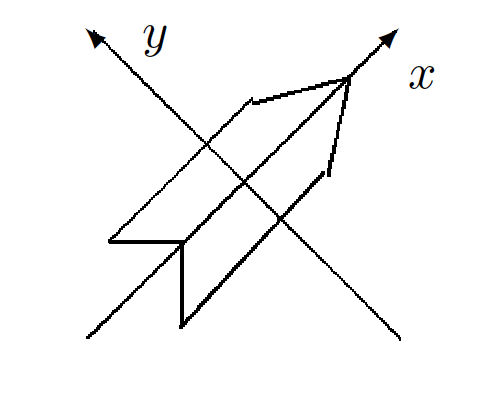
\includegraphics[scale=0.5]{PIC_3.png}
		\\\textbf{Рис. 3:} Пластинка чувствительного оттенка
	\end{center}
	
	Выше предполагалось известным, какому из двух главных направлений пластинки в четверть длины волны соответствует большая скорость распространения света.
	Установить это можно различными способами, например с помощью
	пластинки чувствительного оттенка (так называют пластинку в $ \lambda $
	для зелёной спектральной компоненты, $ \lambda = 560 $ нм).
	
	Пластинка имеет форму стрелы (рис. 3), вдоль оси которой расположено главное направление, соответствующее большей скорости распространения.
	
	\newpage
	
	%Страница 5
	
	\begin{flushleft}
		\footnotesize{Поляризация} \hspace{\fill} \footnotesize{5}
		\\[-0.3cm]\noindent\rule{\textwidth}{0.3pt}
	\end{flushleft}
	
	Если пластинка чувствительного оттенка помещена между скрещенными поляроидами и главные направления пластинки не параллельны
	направлениям разрешённых колебаний поляроидов, то при освещении
	белым светом пластинка кажется окрашенной в лилово-красный цвет.
	Это объясняется тем, что зелёная компонента линейно поляризованного света при прохождении пластинки не меняет поляризации и задерживается вторым поляроидом. Для красной и фиолетовой компонент
	пластинка создаёт сдвиг фаз, несколько отличный от $ 2\pi $. На выходе
	из пластинки красная и фиолетовая компоненты оказываются поэтому
	эллиптически поляризованными и частично проходят через второй поляроид. Таким образом, в известном смысле наблюдаемый в указанном
	опыте цвет пластинки дополнителен к зелёному.
	
	Если между скрещенными поляроидами поместить пластинку чувствительного оттенка
	($ \lambda $) и пластинку в $ \lambda/4 $ так, чтобы их главные
	направления совпадали, цвет пластинки изменится. Если у пластинки чувствительного оттенка и пластинки в $ \lambda/4  $ совпадут главные направления, соответствующие большей скорости распространения, то разность хода между $ E_x $ и $ E_y $ для зелёного света составит уже $ 5\lambda/4 $. Это соответствует разности хода в $ \lambda $ для света с большей длиной волны, т. е. для "<более красного"> света. При освещении
	этих пластинок (напомним, что они расположены между скрещенными поляроидами) белым светом теперь погасится не зелёная, а красная
	часть спектра, и проходящий свет будет казаться зеленовато-голубым.
	Если же главные направления, соответствующие большей скорости распространения, у пластинки чувствительного оттенка и у пластинки
	в $ \lambda/4 $ окажутся перпендикулярными, то проходящий свет приобретёт
	оранжево-желтую окраску (погасится фиолетово-голубая часть спектра).
	
	Изменение цвета позволяет, таким образом, определить, какое из
	главных направлений пластинки в $ \lambda/4 $ соответствует большей скорости
	распространения.
	
	
	\subsection{Интерференция поляризованных лучей}
	
	\begin{center}
		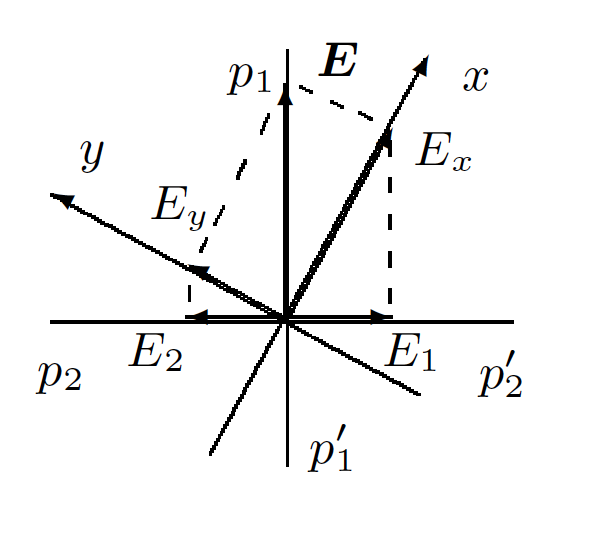
\includegraphics[scale=0.5]{PIC_4.png}
		\\\textbf{Рис. 4:} К объяснению интерференции поляризованных лучей
	\end{center}
	
	Тонкие двоякопреломляющие пластинки, помещённые между поляроидами, кажутся окрашенными. Эта окраска может быть истолкована как результат интерференции поляризованных лучей. На рис. 4 представлена схема для
	случая скрещенных поляроидов.
	
	Здесь $ p1p'1 $ --- разрешённое направление колебаний поляризатора
	(первого поляроида); $ x, y $ --- координатная система, связанная с главными направлениями двоякопреломляющей пластинки; $ p2p'2 $ --- разрешённое направление колебаний анализатора (второго поляроида). Волны
	$ E_x  $ и $ E_y $ на выходе из пластинки когерентны, но не могут интерферировать, так как $ E_x \perp  E_y $. Волны $ E_1 $ и $ E_2 $ на выходе второго поляроида
	также являются когерентными и к тому же поляризованы в одной плоскости. Эти волны интерферируют между собой. Результат интерференции определяется зависящим от длины волны сдвигом фаз между $ E_1 $
	и $ E_2 $. В результате интерференции поляризованных лучей пластинка, освещаемая белым светом, кажется окрашенной.
	
	\newpage
	
	%Страница 6
	
	\begin{flushleft}
		\footnotesize{Поляризация} \hspace{\fill} \footnotesize{6}
		\\[-0.3cm]\noindent\rule{\textwidth}{0.3pt}
	\end{flushleft}
	
	Если поворачивать двоякопреломляющую пластинку, расположенную между
	скрещенными поляроидами, то соотношение амплитуд волн $ E_1 $ и $ E_2 $ и разность фаз между ними не изменяются. Это означает, что цвет пластинки при её поворотах не меняется, а меняется только интенсивность света. За один оборот пластинки интенсивность четыре раза обращается в нуль --- это происходит при совпадении главных направлений
	$ x $ и $ y $ с разрешёнными направлениями колебаний поляроидов.
	
	Если же двоякопреломляющую пластинку оставить неподвижной, а
	второй поляроид повернуть так, чтобы разрешённые направления $ p1p'1 $
	и $ p2p'2 $ совпали, то волны $ E_1 $ и $ E_2 $ приобретают дополнительный фазовый сдвиг на $ \pi $ для всех спектральных компонент; при этом их амплитуды изменятся так, что цвет пластинки изменится на дополнительный. 
	
	\section{Проведение эксперимента}
	
	\subsection{Определение разрешенных направлений поляроидов}
	
	\begin{center}
		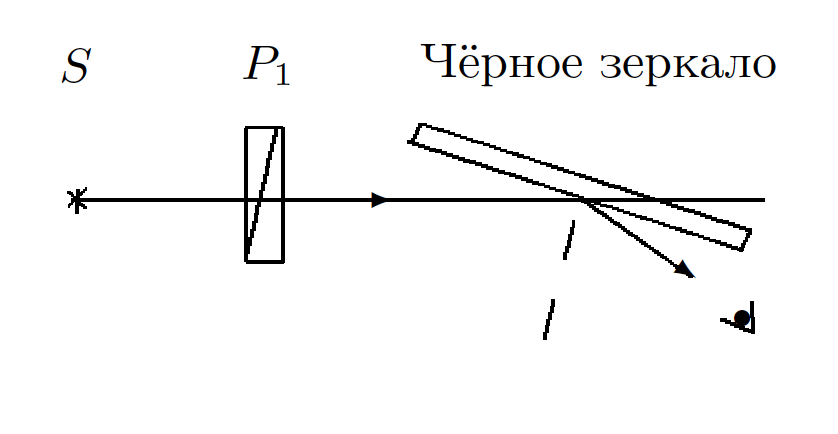
\includegraphics[scale=0.5]{PIC_5.png}
		\\\textbf{Рис. 5:} Определение разрешенных направлений поляроидов
	\end{center}
	
	Поворачивая поляроид вокруг направления луча, а чёрное зеркало вокруг вертикальной оси, методом последовательных приближений добьемся
	наименьшей яркости отражённого пятна. Определим разрешённое направление поляроида. По лимбу оно равно $ \psi_1 = 126^\circ $. 
	
	Поставим вместо чёрного зеркала второй поляроид и определим
	его разрешённое направление, скрестив поляроиды. Получаем $ \psi_2 = 347^\circ $. 
	
	\subsection{Определение показателя преломления эбонита}
	
	Поставим на скамью вместо чёрного зеркала (рис. 5) эбонитовую пластину, ее "<ноль"> по лимбу на $\theta_1 = 40^\circ$. Определим по лимбу наименьшую яркость пятна, она на отметке $\theta_2 = (95 \pm 2)^\circ$. Тогда искомый угол Брюстера $\theta_{\text{бр}} = (55 \pm 2)^\circ$. Наконец, показатель преломления эбонита:
	
	$$n_{\text{эб}} = 1.43 \pm 0.11$$
	
	Повторение эксперимента с зеленым светофильтром дает тот же результат в пределах погрешности.
	
	\subsection{Исследование стопы}
	
	\begin{center}
		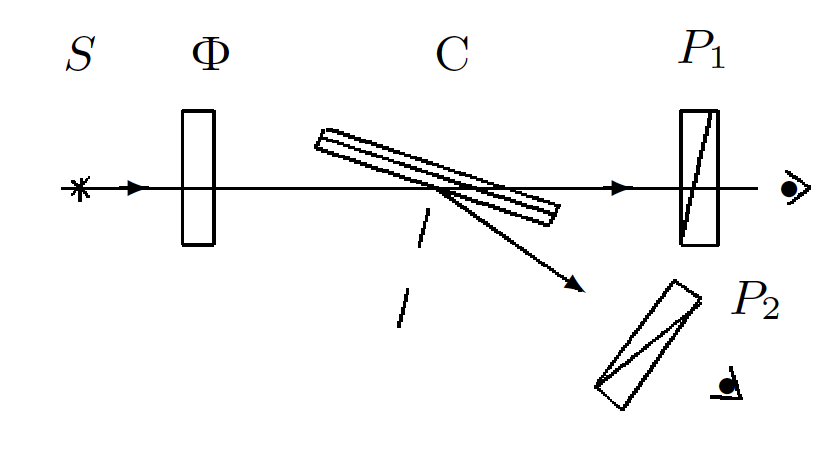
\includegraphics[scale=0.45]{PIC_6.png}
		\\\textbf{Рис. 6:} Исследование стопы
	\end{center}
	
	\newpage
	
	%Страница 7
	
	\begin{flushleft}
		\footnotesize{Поляризация} \hspace{\fill} \footnotesize{7}
		\\[-0.3cm]\noindent\rule{\textwidth}{0.3pt}
	\end{flushleft}
	
	Исследуем характер поляризации света в преломлённом и отражённом от стопы лучах. 
	
	Для этого поставим вместо эбонитового зеркала (рис. 5) стопу стеклянных пластинок под углом Брюстера.
	
	Осветим стопу неполяризованным светом и, рассматривая через поляроиды (рис. 6) отражённый от стопы и преломлённый лучи, определим в них ориентацию вектора $ \vec{E} $. При осмотре отраженного луча через "<вертикальный"> поляроид, изображение видно, при этом оно не видно через "<горизонтальный">. При осмотре преломленного луча ситуация ровно противоположная. Таким образом, в отраженном луче вектор $\vec{E}$ колеблется в плоскости, перпендикулярной плоскости падения, а в преломленном в плоскости падения.
 	
 	\subsection{Двоякопреломляющие пластины}
 	
 	Определим главные направления двоякопреломляющих пластин. 
 	
 	Поставим кристаллическую пластинку между скрещенными поляроидами (рис. 7). Вращая пластинку вокруг направления луча, видим, что минимумы яркости следуют с интервалом в $90^\circ$, что очевидно, так как ровно в этих случаях поляризация света остается неизменной.
 	
 	\begin{center}
 		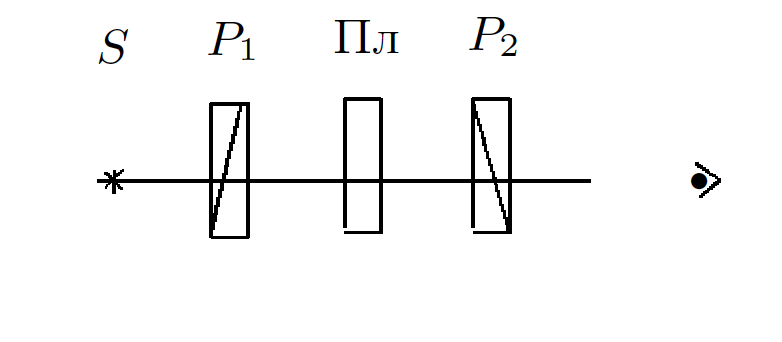
\includegraphics[scale=0.5]{PIC_7.png}
 		\\\textbf{Рис. 7:} Исследование двоякопреломляющих пластин
 	\end{center}
 	
 	Для другой из пластинок наблюдается аналогичное. Для пластинки 3 один из минимумов $\psi_3 = 120^\circ$, для пластинки 3' такой $\psi_4 = 80^\circ$.
 	
 	\subsection{Пластинки $ \lambda/2, \lambda/4 $}
 	
 	Для выделения пластин $ \lambda/2, \lambda/4 $ добавим к схеме, изображённой на рис. 7, зелёный фильтр и установим разрешённое направление первого поляроида горизонтально, а главные направления исследуемой пластинки --- под углом $ 45^\circ $ к горизонтали.
 	
 	C помощью второго поляроида установим, какую поляризацию
 	имеет свет, прошедший пластинку: круговую или линейную с переходом
 	в другой квадрант. Для пластинки 3 наблюдается заметное изменение яркости при повороте выходного поляроида, что свидетельствует о линейной поляризации, то есть \textbf{пластинка 3 это полуволновая пластинка}. Для пластинки 3' изменения яркости практически не наблюдается, значит, поляризация круговая и \textbf{пластинка 3' четвертьволновая.}
 	
 	\subsection{Быстрая и медленная оси $ \lambda/4 $}.
 	
 	 \begin{center}
 		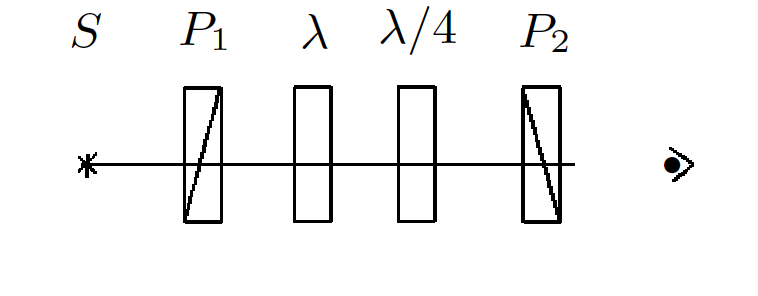
\includegraphics[scale=0.5]{PIC_8.png}
 		\\\textbf{Рис. 8:} Исследование четвертьволновой пластинки
 	\end{center}
 	
 	\newpage
 	
 	%Страница 8
 	
 	\begin{flushleft}
 		\footnotesize{Поляризация} \hspace{\fill} \footnotesize{8}
 		\\[-0.3cm]\noindent\rule{\textwidth}{0.3pt}
 	\end{flushleft}
 	
 	В условиях предыдущего опыта эта пластинка в самом деле не меняет поляризации зеленого света. В нашем же опыте без светофильтра стрелка выглядит пурпурной. (Объяснение в теорсправке)
 	
 	Поставим теперь четвертьволновую пластинку. Пронаблюдаем за ее цветами:
 	
 	\begin{figure}[h]
 		\begin{minipage}{0.5\linewidth}
 			\begin{center}
 				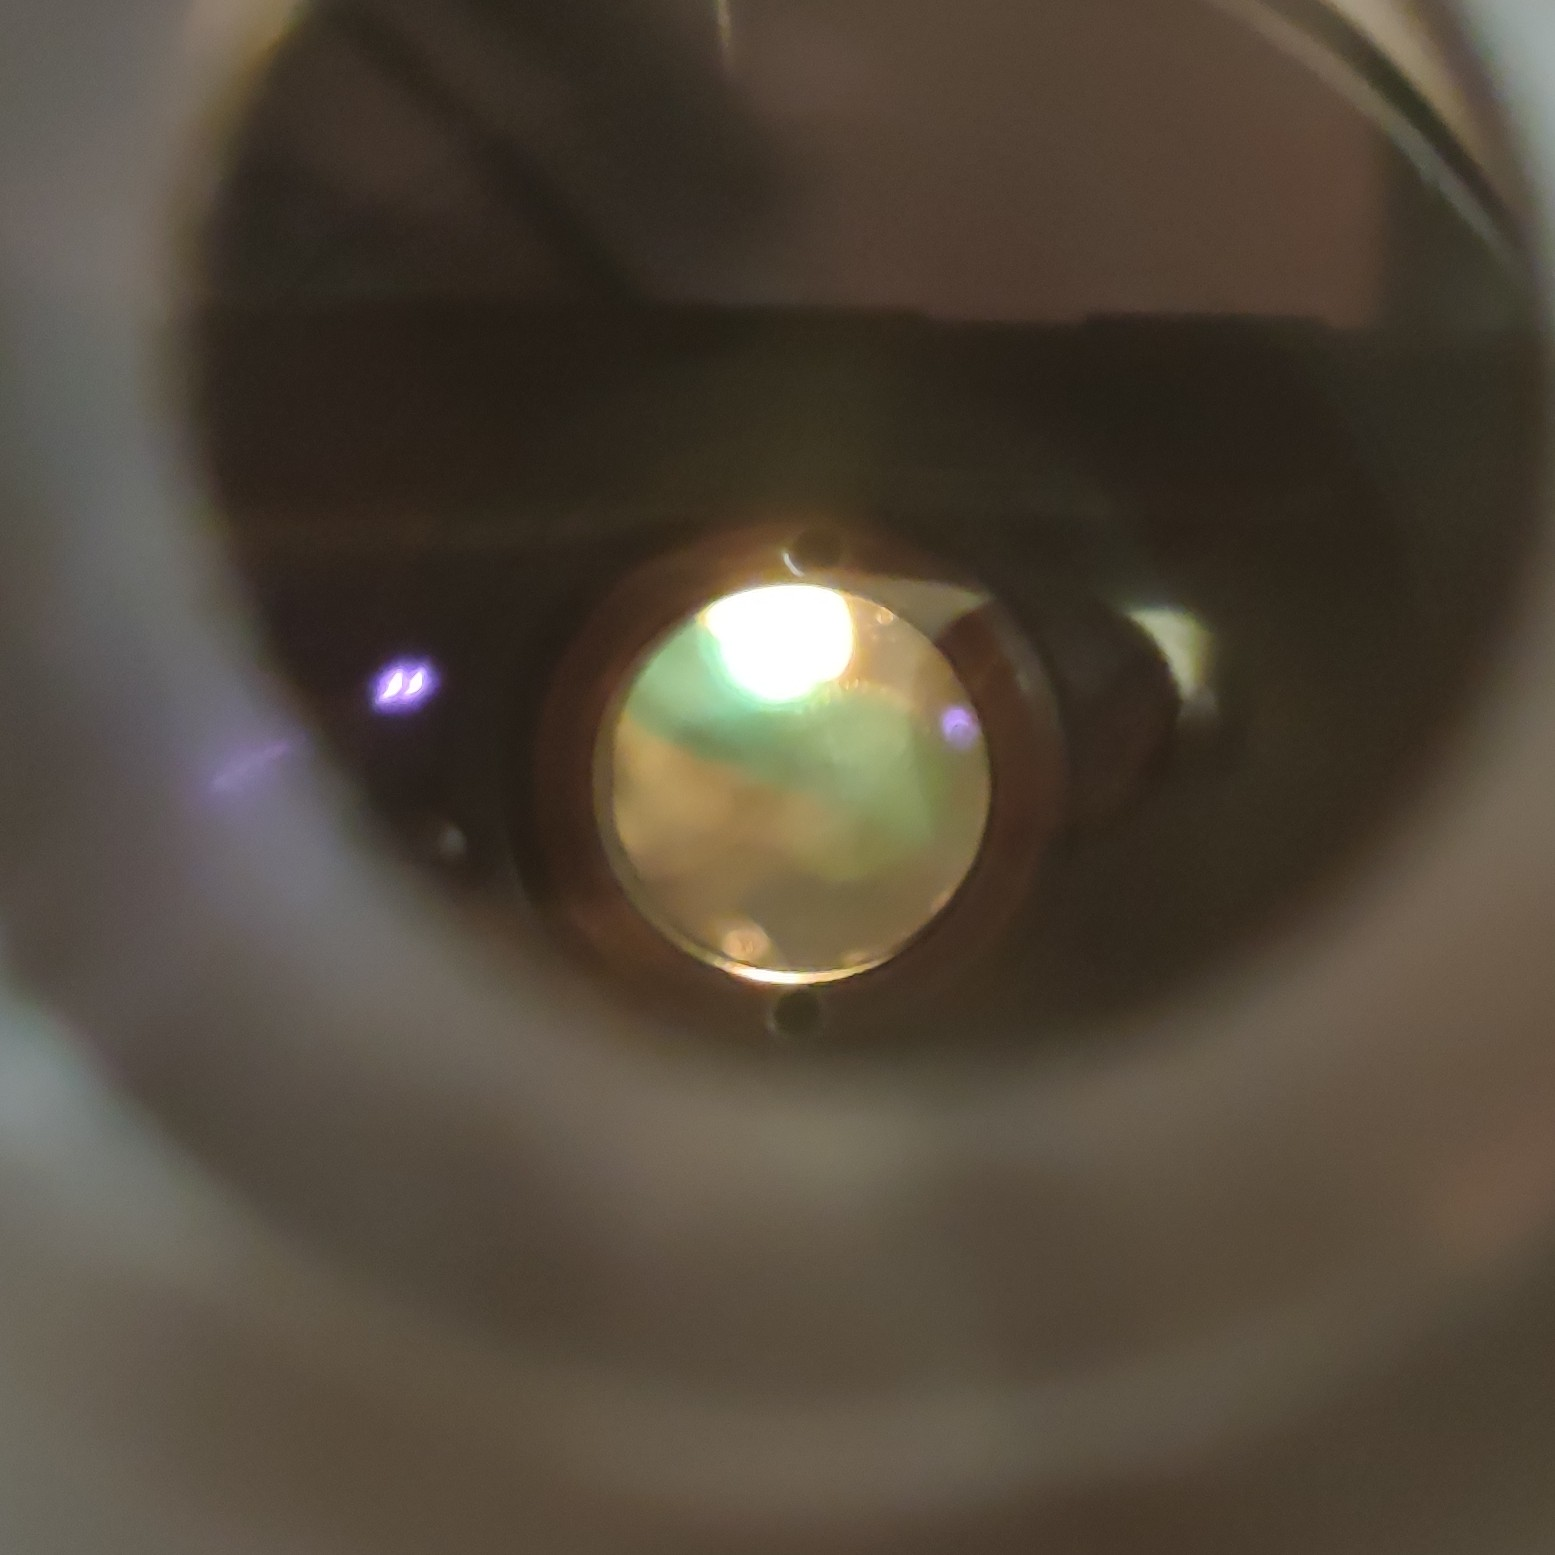
\includegraphics[scale=0.111]{PIC_9.jpg}
 			\end{center}
 		\end{minipage}
 		\begin{minipage}{0.5\linewidth}
 			 \begin{center}
 				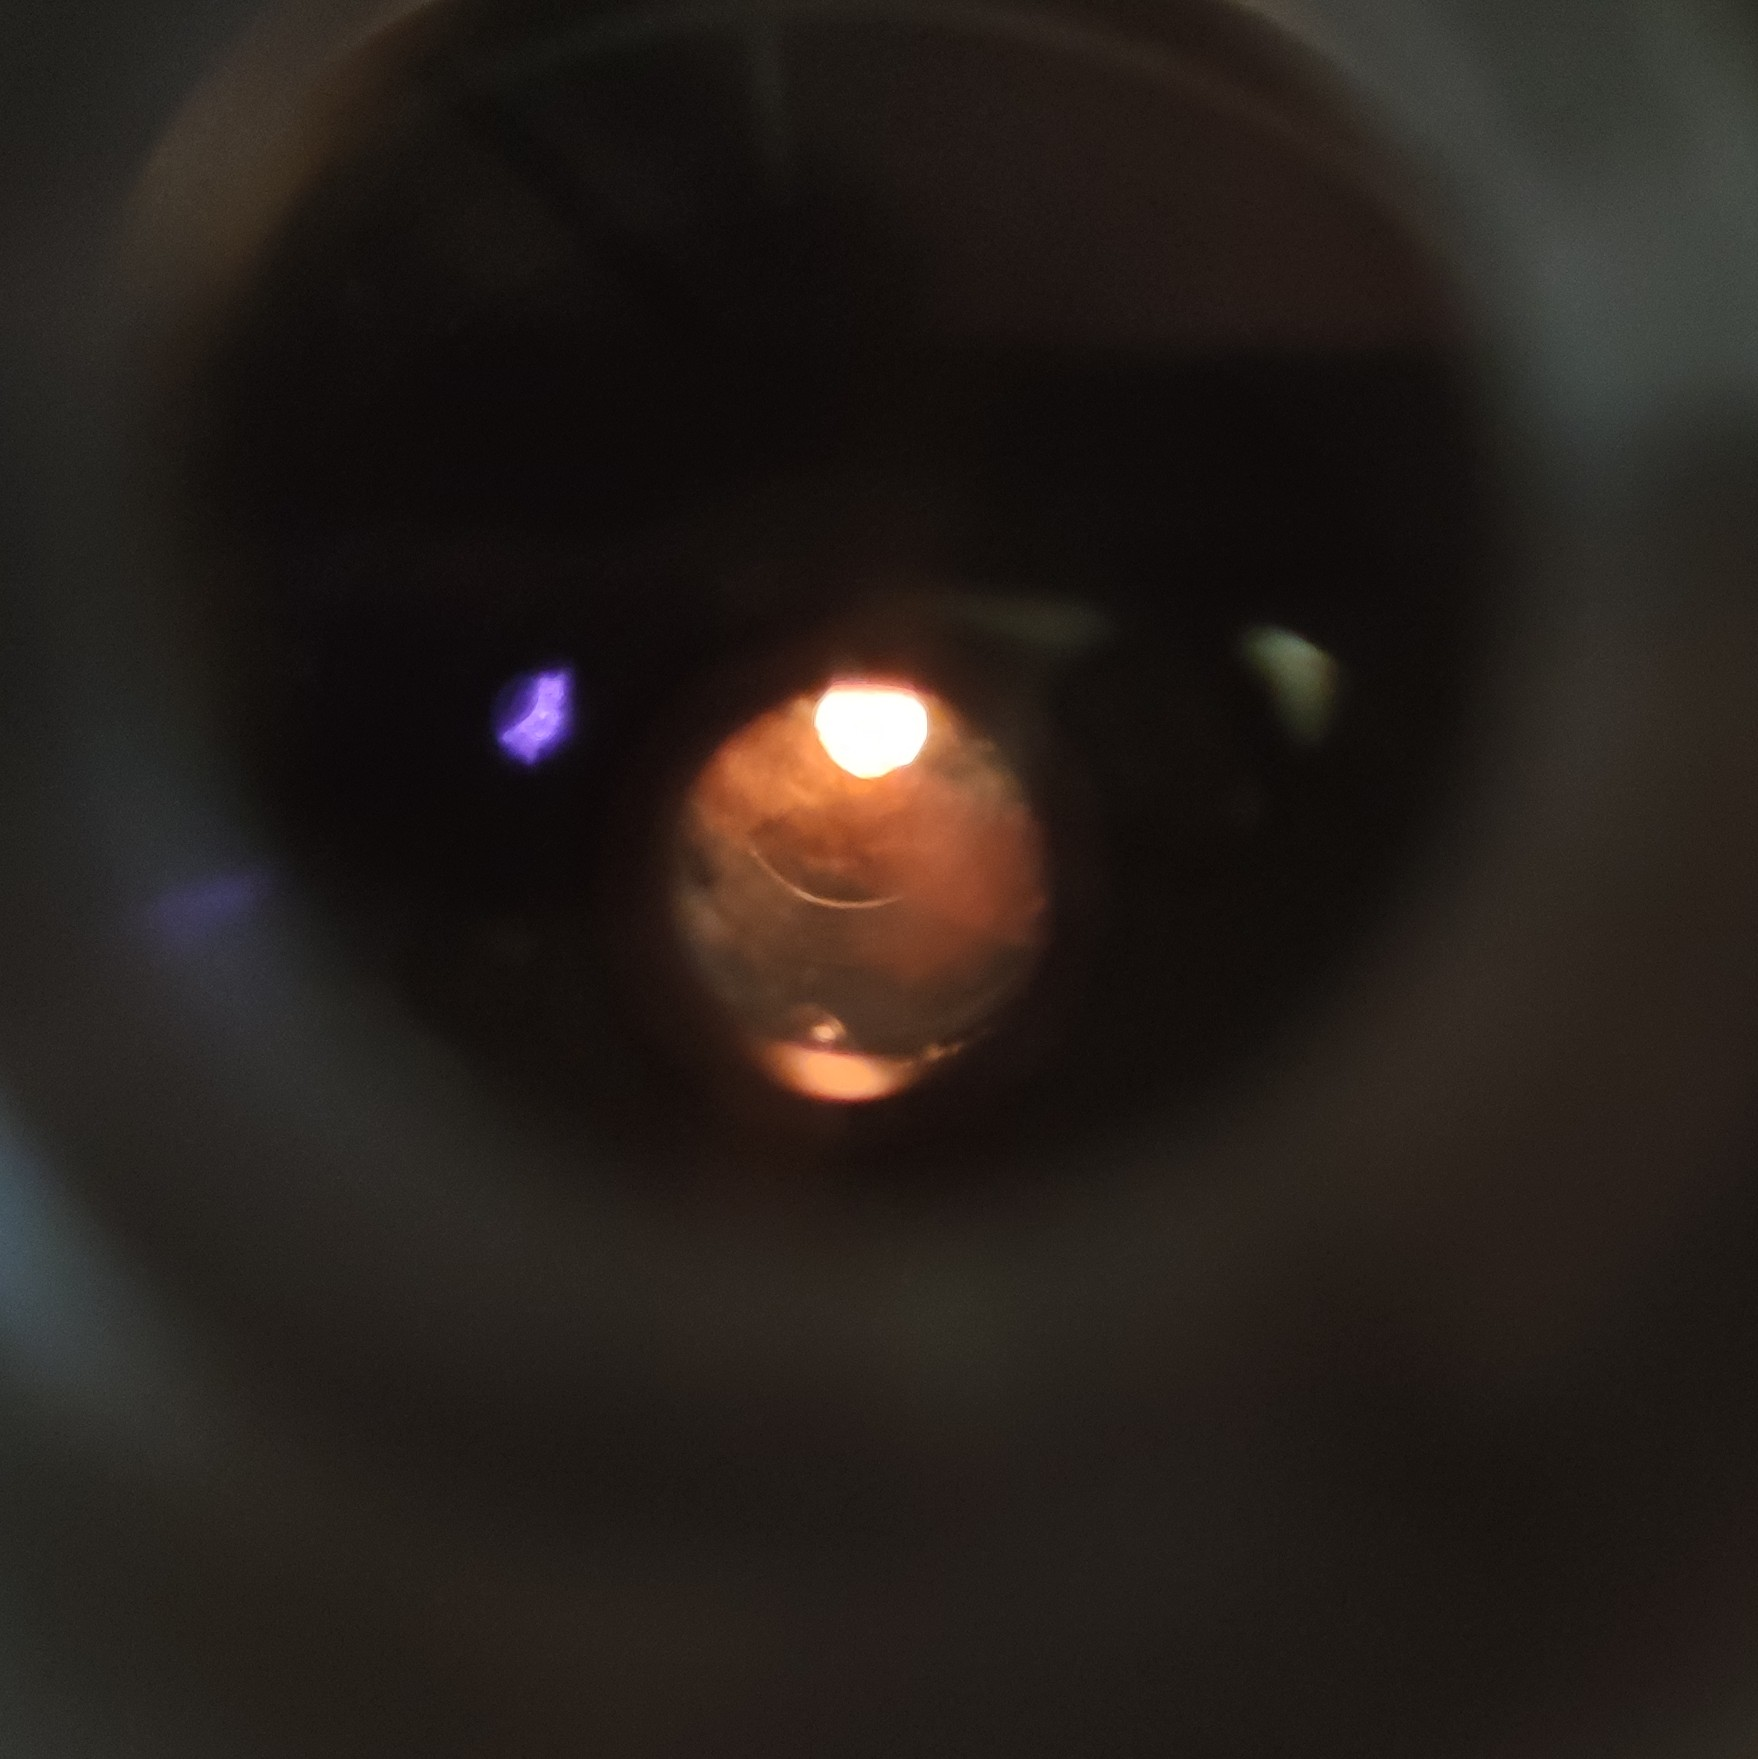
\includegraphics[scale=0.1]{PIC_10.jpg}
 			\end{center}
 		\end{minipage}
 		\begin{center}
 			\textbf{Рис. 9-10:} Пластинка чувствительного оттенка
 		\end{center}
 	\end{figure}
 	
 	По наблюдаемым результатам делаем вывод, что рисунок 9 соответствует быстрой оси четвертьволновой пластинки, а рисунок 10 -- медленной.
 	
 	\subsection{Интерференция поляризованных лучей}
 	
 	Исследуем интерференцию поляризованных лучей. Для этого расположим между скрещенными поляроидами мозаичную слюдяную пластинку. Она собрана из 4-х узких полосок слюды, лежащих по сторонам
 	квадрата (две полоски "<толщиной"> $ \lambda/4 $ и по одной --- $ \lambda/2 $ и $ 3\lambda/4 $). В центральном квадратике слюды нет. Главные направления всех пластинок ориентированы параллельно сторонам квадрата.
 	
 	
 	 \begin{figure}[h]
 		\begin{minipage}{0.3333\linewidth}
 			\begin{center}
 				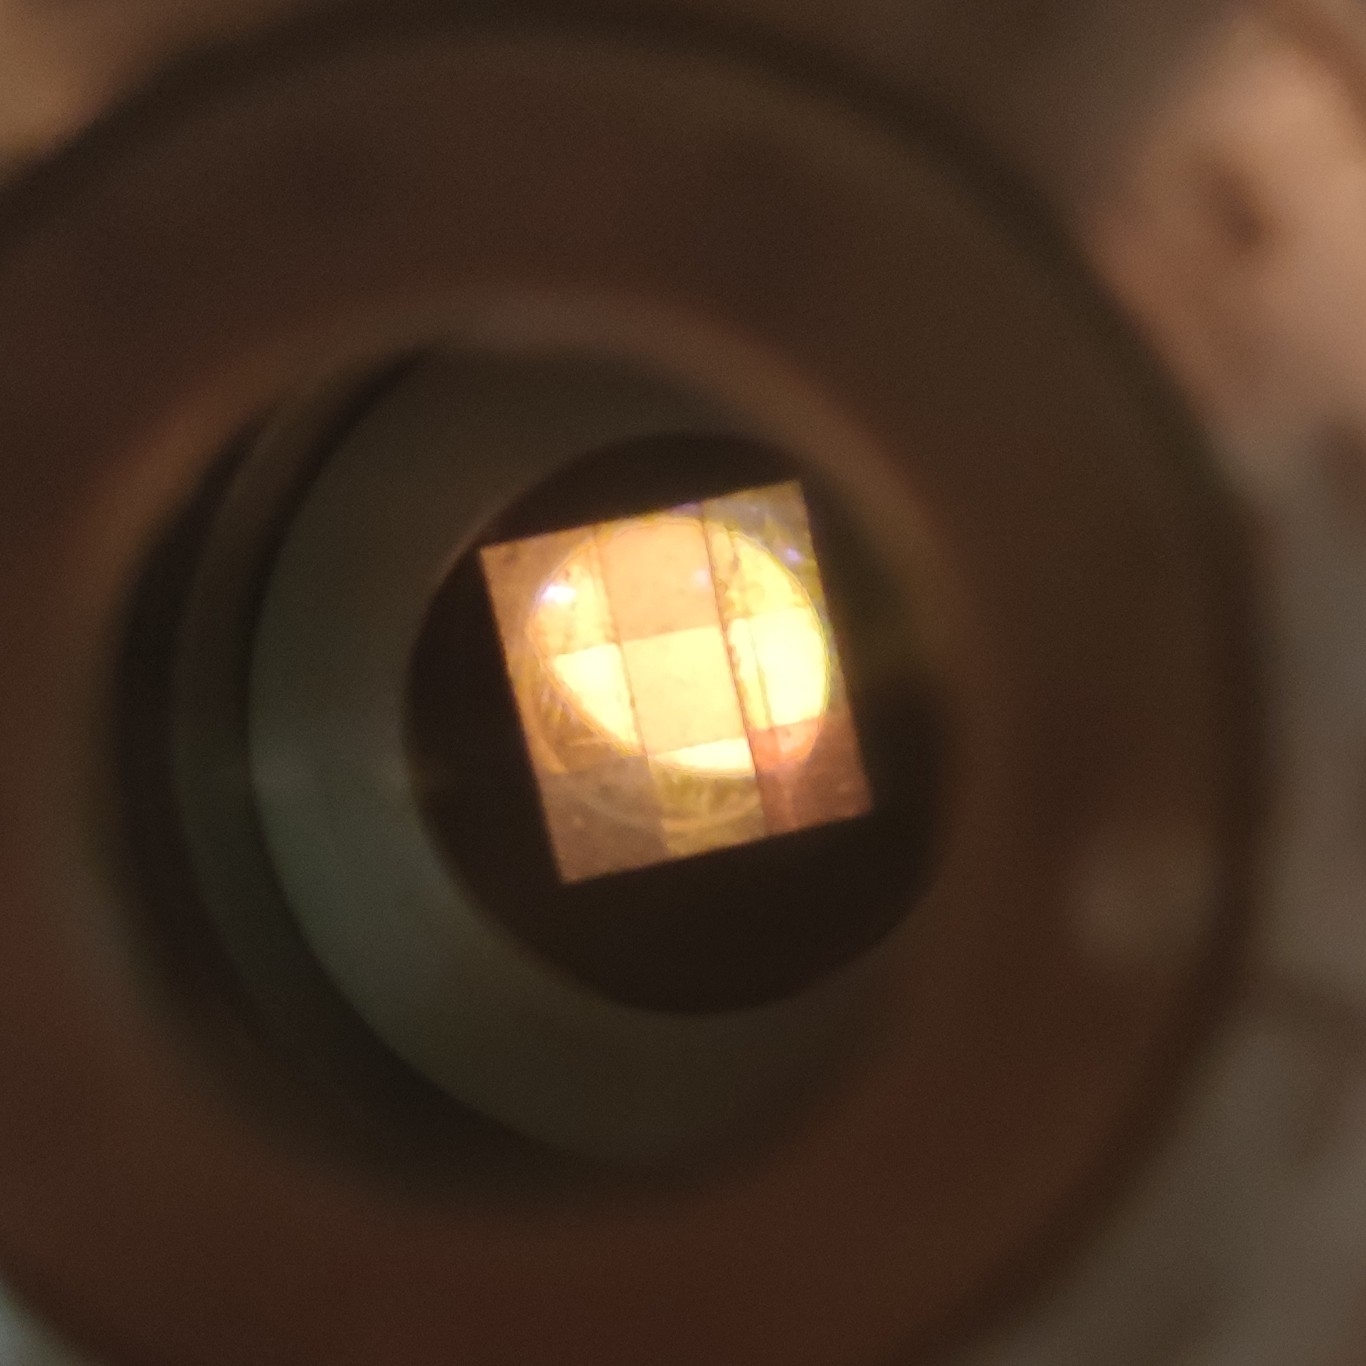
\includegraphics[scale=0.107]{PIC_11.jpg}
 			\end{center}
 		\end{minipage}
 		\begin{minipage}{0.3333\linewidth}
 			\begin{center}
 				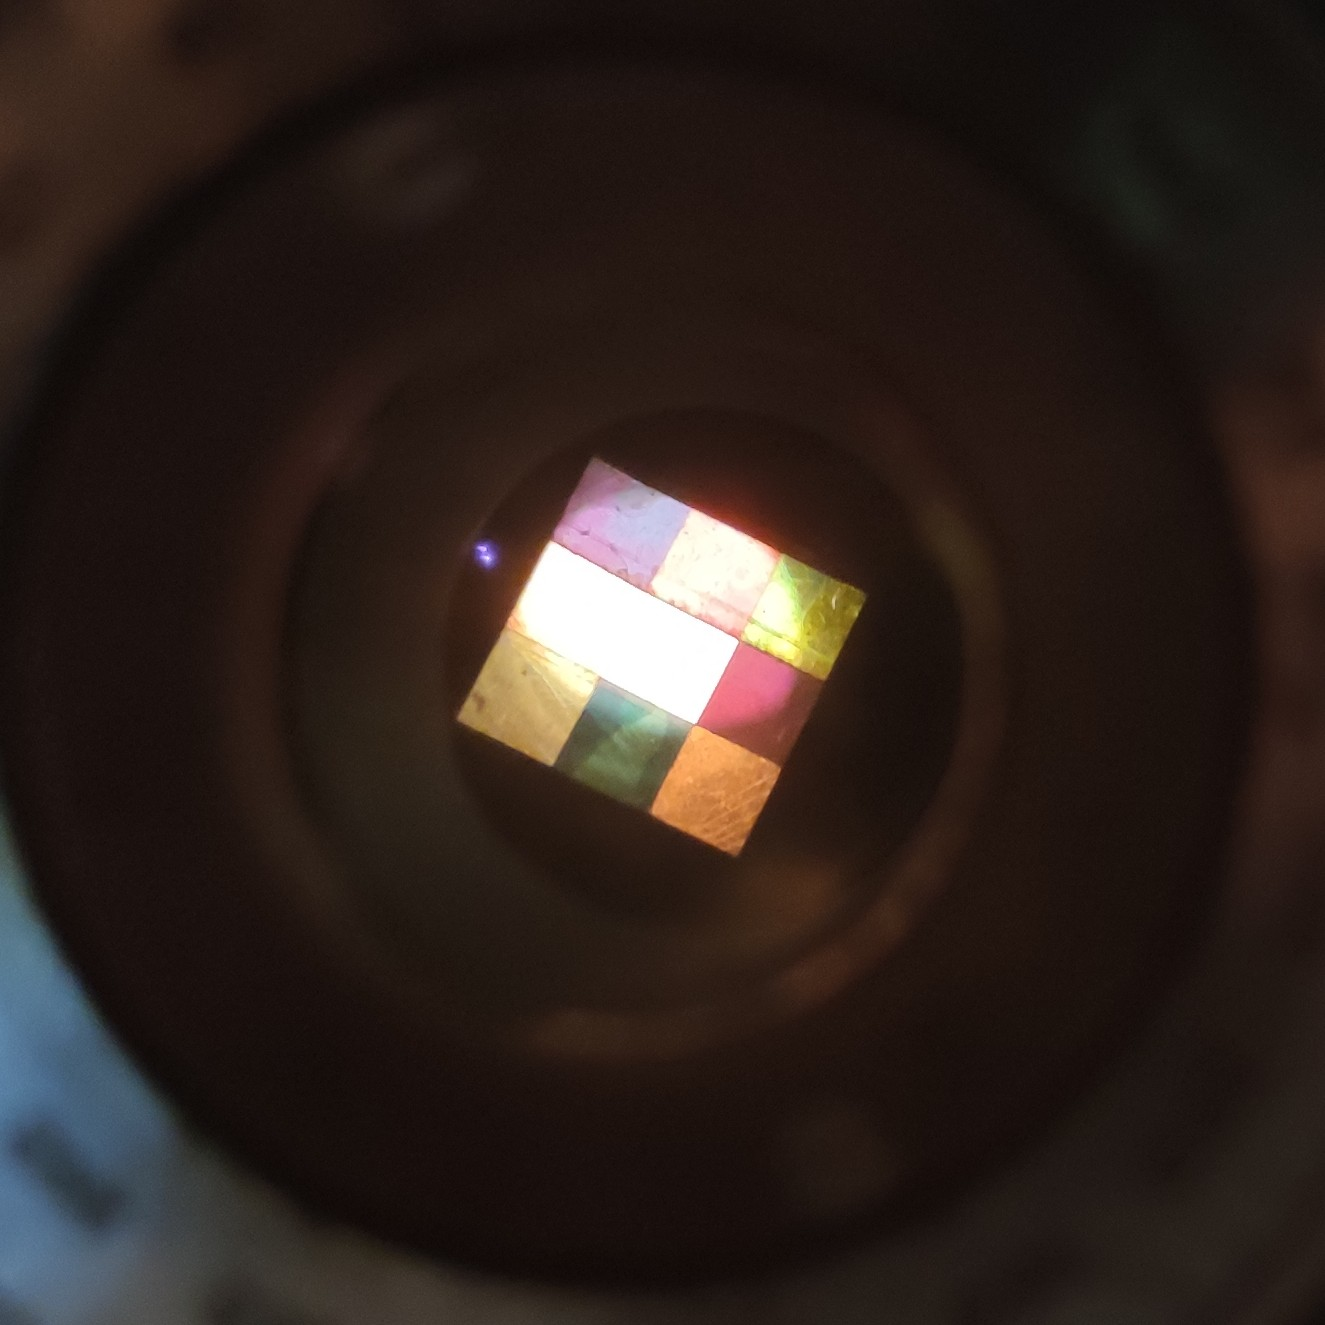
\includegraphics[scale=0.1105]{PIC_12.jpg}
 			\end{center}
 		\end{minipage}
 		\begin{minipage}{0.3333\linewidth}
 			\begin{center}
 				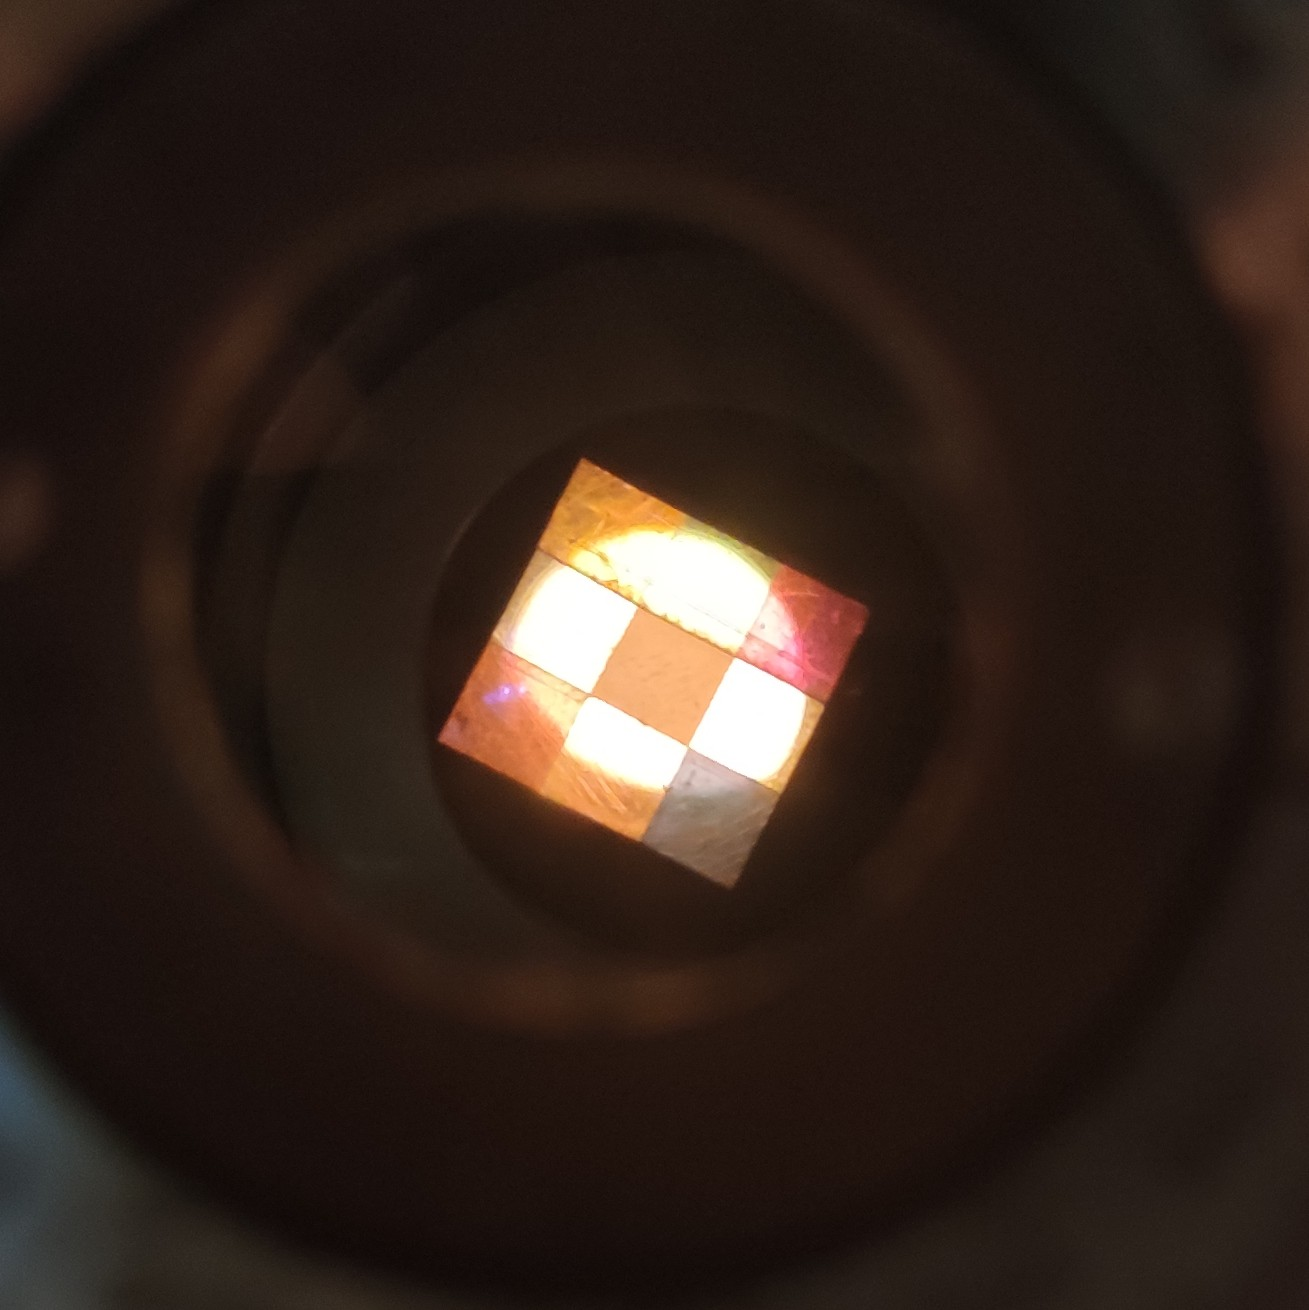
\includegraphics[scale=0.111]{PIC_13.jpg}
 			\end{center}
 		\end{minipage}
 		\begin{center}
 			\textbf{Рис. 11-13:} Слюдяная мозаичная пластинка
 		\end{center}
 	\end{figure}
 	
 	
 	Вращая пластинку, пронаблюдаем за изменениями в отдельном квадратике (рис. 11-12). У нас изменяется интенсивность 4 раза за период, поскольку главные оси пластинок совпадают с осями поляроидов.
 	
 	Не трогая пластинки, повращаем второй поляроид (рис.12-13). Теперь наблюдаем изменение цветов. 
 	
	\newpage
	
	%Страница 9
	
	\begin{flushleft}
		\footnotesize{Поляризация} \hspace{\fill} \footnotesize{9}
		\\[-0.3cm]\noindent\rule{\textwidth}{0.3pt}
	\end{flushleft}

	\subsection{Эллиптически поляризованная волна}

	Нарисуем эллипс поляризации для вектора напряжённости из пластинки $ \lambda/4 $ и укажем, какая из осей соответствует большей скорости. На нашем рисунке это ось $ x $.
	
	Рядом нарисуем две вышедших из пластинки синусоиды: $ x(t) $ и $ y(t) $ со сдвигом фаз в четверть периода. 
	
	Определим направление вращения электрического вектора в эллиптически поляризованной волне, указав его стрелкой на соответствующем рисунке.
	
	 \begin{figure}[h]
		\begin{minipage}{0.5\linewidth}
			\begin{center}
				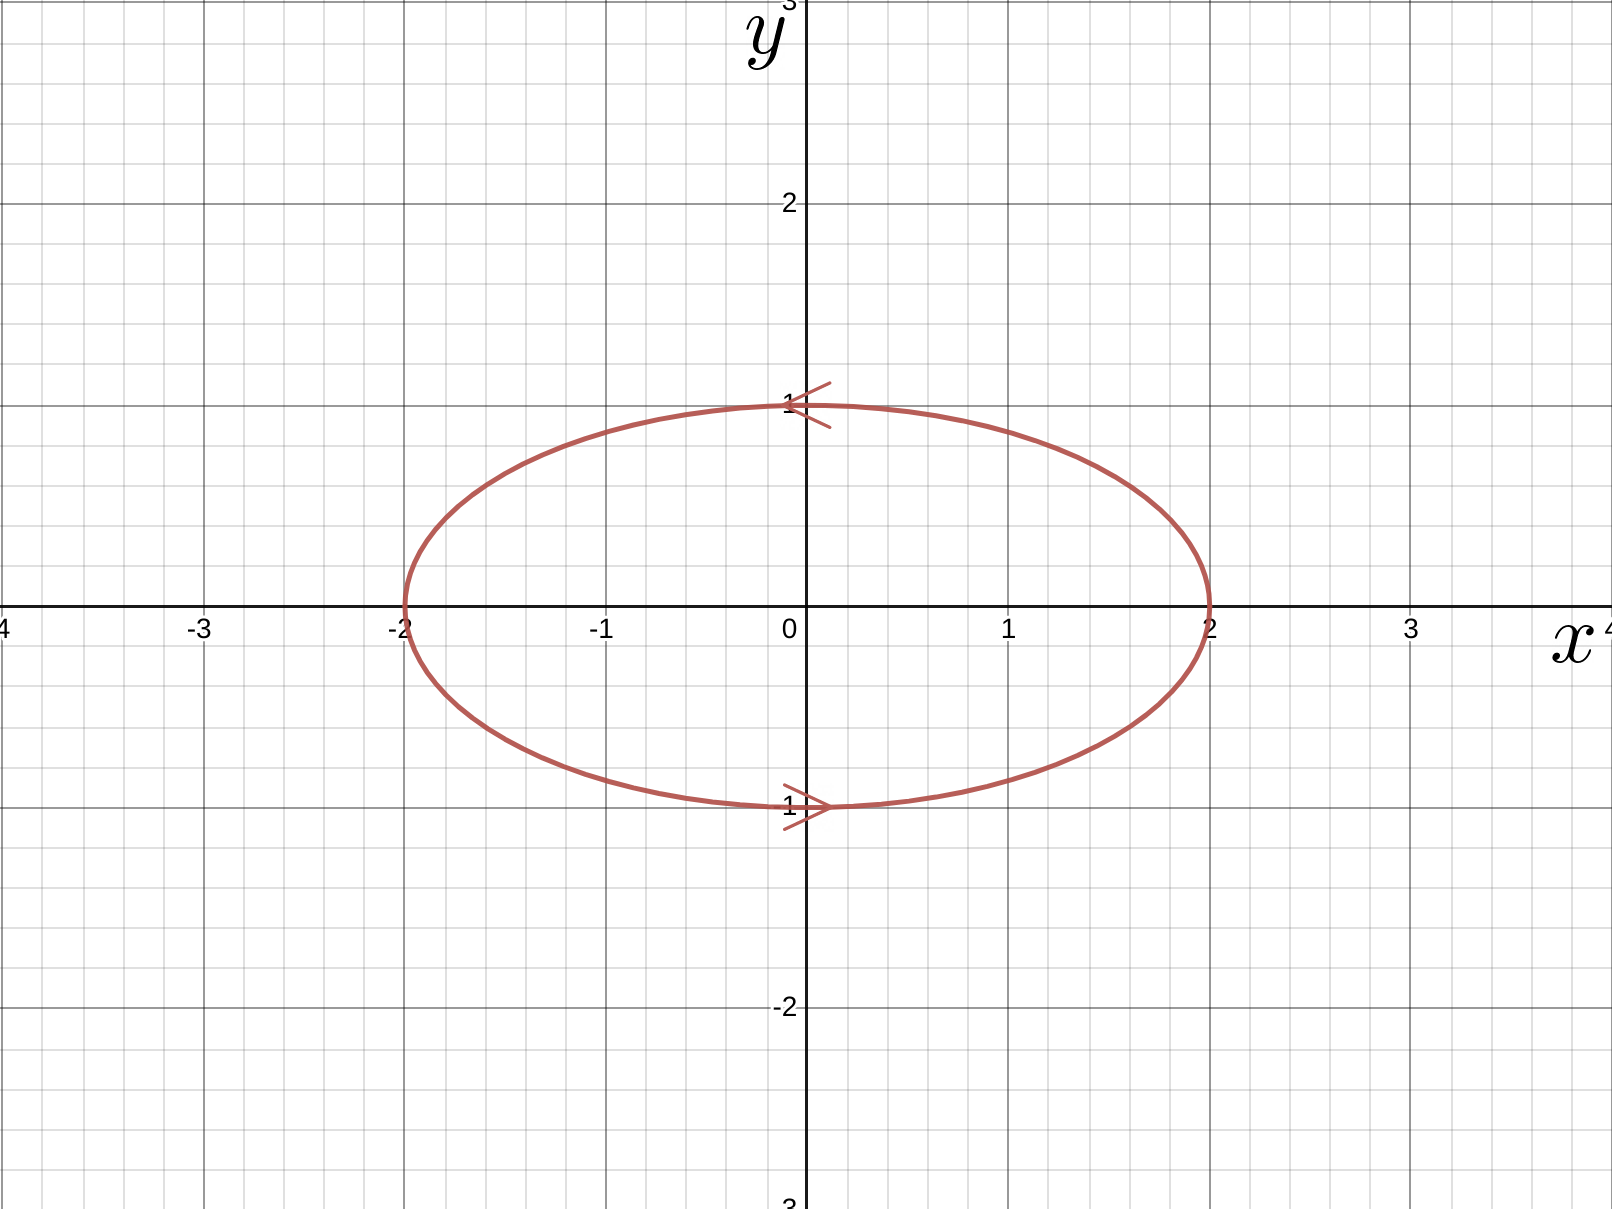
\includegraphics[scale=0.12]{PIC_14.png}
			\end{center}
		\end{minipage}
		\begin{minipage}{0.5\linewidth}
			\begin{center}
				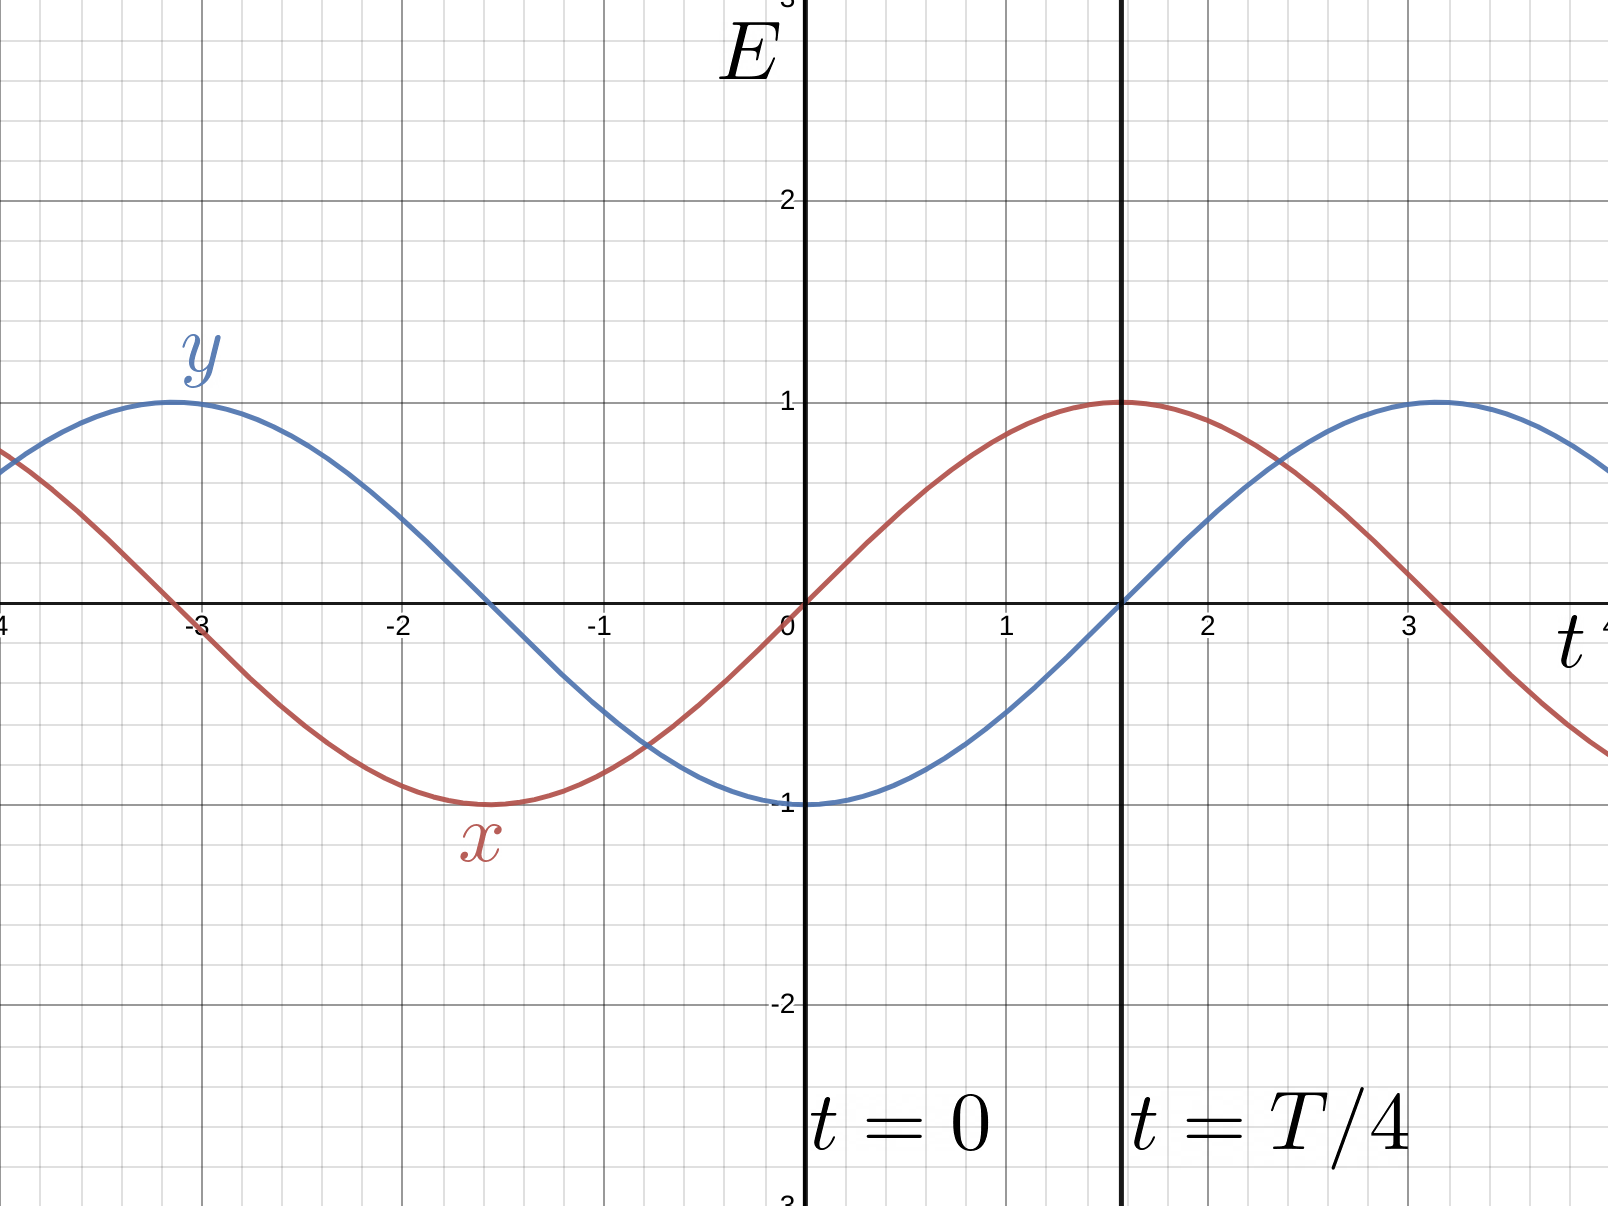
\includegraphics[scale=0.12]{PIC_15.png}
			\end{center}
		\end{minipage}
		\begin{center}
			\textbf{Рис. 14-15:} Эллиптически поляризованная волна
		\end{center}
	\end{figure}

	Снова поставим зелёный фильтр, а за ним между скрещенными поляроидами --- пластинку произвольной толщины.

	Получили эллиптически-поляризованный свет. Для этого установили разрешённое направление первого поляроида под углом 10–20$^\circ$ к горизонтали так, чтобы вектор $\vec{E}$ падающего на пластинку света был расположен в первом квадранте. Установили разрешённое направление второго поляроида вертикально и, вращая пластинку, нашли минимальную интенсивность света, прошедшего второй поляроид. Вращая второй поляроид, убедились, что свет поляризован эллиптически, а не линейно. Таким образом получили эллипс поляризации с вертикально ориентированной малой осью.
	
	\begin{figure}[h]
		\begin{minipage}{0.5\linewidth}
			\begin{center}
				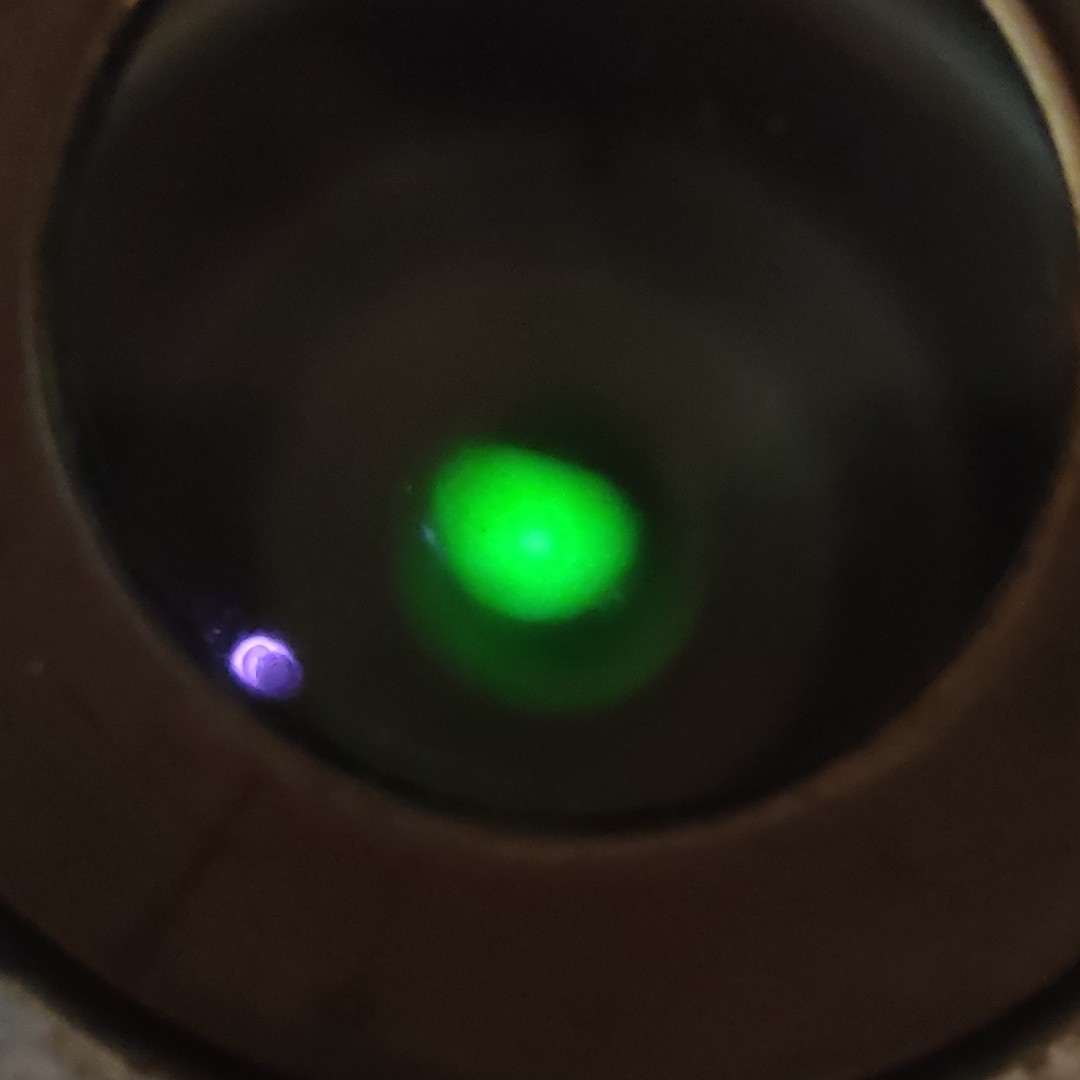
\includegraphics[scale=0.13]{PIC_16.jpg}
			\end{center}
		\end{minipage}
		\begin{minipage}{0.5\linewidth}
			\begin{center}
				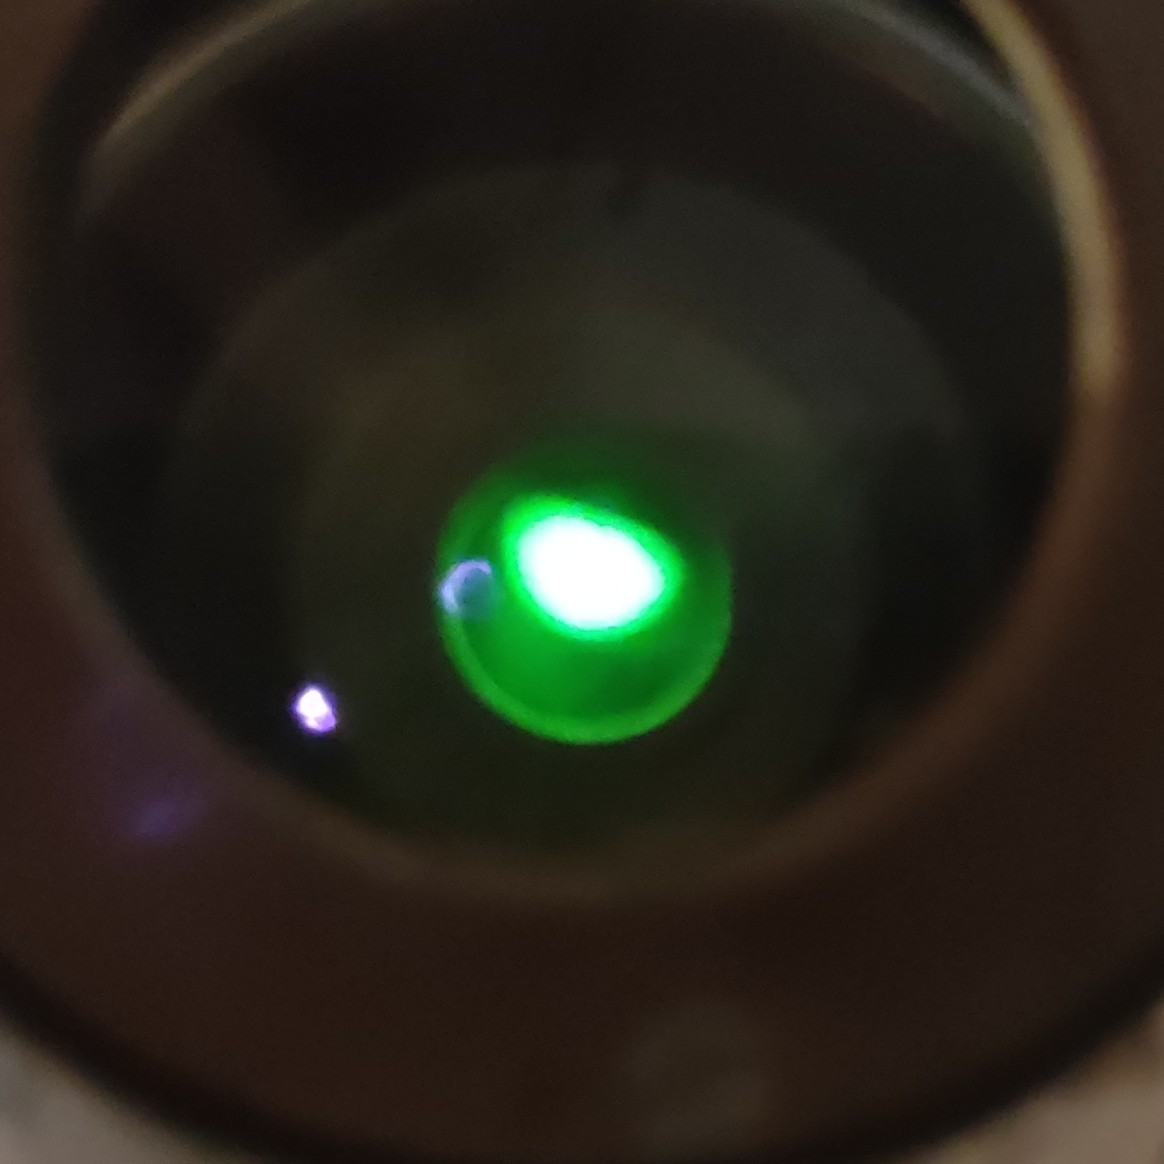
\includegraphics[scale=0.122]{PIC_17.jpg}
			\end{center}
		\end{minipage}
		\begin{center}
			\textbf{Рис. 16-17:} Эллиптически поляризованная волна
		\end{center}
	\end{figure}

	Для определения направления вращения светового вектора в эллипсе 	установили между поляроидами дополнительную пластинку $\lambda/4$ с известными направлениями «быстрой» и «медленной» осей, ориентированными по осям эллипса поляризации анализируемого света. В этом случае вектор $\vec{E}$ на выходе такой, как если бы свет прошёл две пластинки $\lambda/4$: свет на выходе из второй пластинки будет линейно поляризован. Если пластинки поодиночке дают эллипсы, вращающиеся в разные стороны, то поставленные друг за другом, они скомпенсируют разность фаз, и вектор $\vec{E}$ на выходе останется в первом и третьем квадрантах. Если же световой вектор перешёл в смежные квадранты, значит, эллипсы вращаются в одну сторону. А как вращается эллипс в пластинке $\lambda/4$, определили ранее.
	
	\newpage
	
	%Страница 10
	
	\begin{flushleft}
		\footnotesize{Поляризация} \hspace{\fill} \footnotesize{10}
		\\[-0.3cm]\noindent\rule{\textwidth}{0.3pt}
	\end{flushleft}
	
	\section{Выводы}
	
	Изучили явления связанные с поляризацией света:
	
	\begin{itemize}
		\item Определили разрешённые направления поляроидов
		\item Рассмотрели угол Брюстера, с помощью него определили показатель преломления эбонита
		\item Для двоякопреломляющих пластин определили главные направления, а так же тип пластинок --- $\lambda /4$ и $\lambda/2$
		\item Исследовали пластинку чувствительного оттенка, определили быструю и медленную оси пластинки $\lambda/4$ и рассмотрели эффекты, происходящие при прохождении света через комбинацию пластинок
		\item рассмотрели интерференцию поляризованных лучей в мозаичной слюдяной пластинке
		\item Получили эллиптически поляризованную волну
	\end{itemize}
	
\end{document}